\documentclass[border=10pt]{standalone}
\usepackage{tikz}
\usetikzlibrary{shapes, arrows.meta, positioning, calc, fit, backgrounds, shadows}

\begin{document}
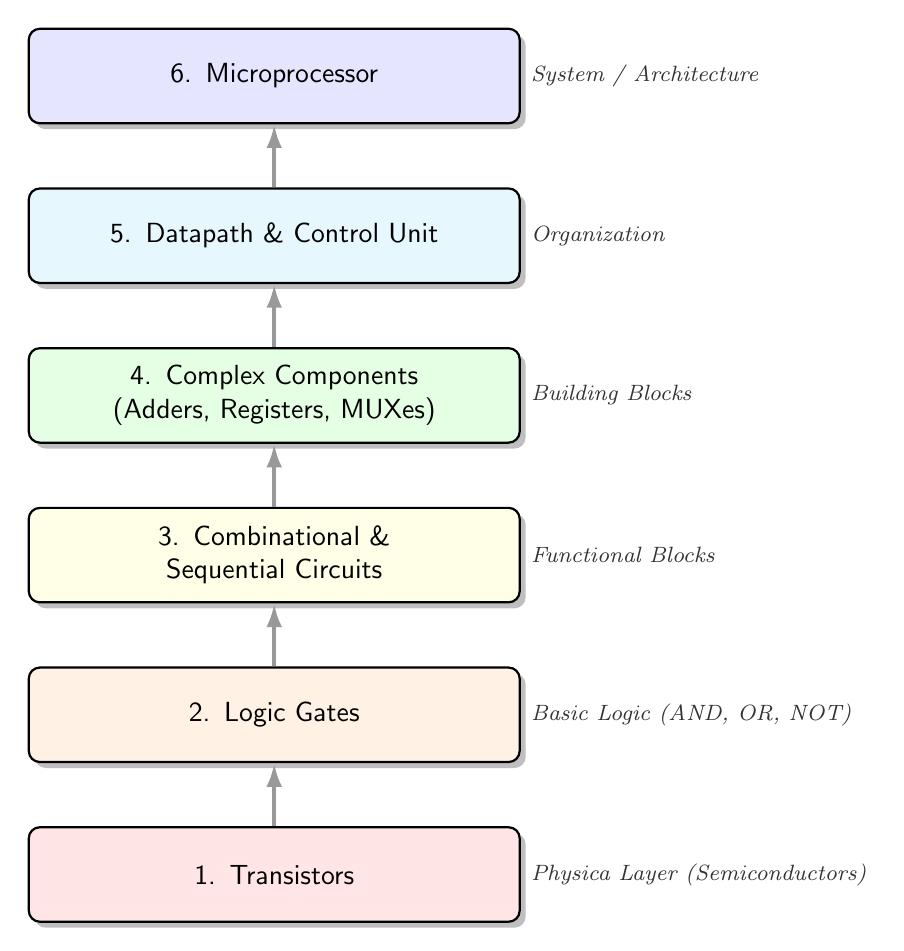
\begin{tikzpicture}[
    font=\sffamily,
    thick,
    level/.style={draw, rounded corners, minimum height=1.2cm, align=center, fill=white, drop shadow, text width=6cm},
    arrow/.style={-{Latex[length=3mm, width=2mm]}, line width=1.5pt, color=gray!80},
    note/.style={font=\footnotesize\itshape, color=gray!40!black, anchor=west}
]

    % Levels
    \node[level, fill=red!10] (transistors) {1. Transistors};
    \node[level, fill=orange!10, above=0.8cm of transistors] (gates) {2. Logic Gates};
    \node[level, fill=yellow!10, above=0.8cm of gates] (circuits) {3. Combinational \&\\Sequential Circuits};
    \node[level, fill=green!10, above=0.8cm of circuits] (components) {4. Complex Components\\(Adders, Registers, MUXes)};
    \node[level, fill=cyan!10, above=0.8cm of components] (datapath) {5. Datapath \& Control Unit};
    \node[level, fill=blue!10, above=0.8cm of datapath] (microprocessor) {6. Microprocessor};

    % Connections (Upward flow)
    \draw[arrow] (transistors) -- (gates);
    \draw[arrow] (gates) -- (circuits);
    \draw[arrow] (circuits) -- (components);
    \draw[arrow] (components) -- (datapath);
    \draw[arrow] (datapath) -- (microprocessor);

    % Side Notes (Optional, can be removed or refined)
    \node[note] at (transistors.east) {Physica Layer (Semiconductors)};
    \node[note] at (gates.east) {Basic Logic (AND, OR, NOT)};
    \node[note] at (circuits.east) {Functional Blocks};
    \node[note] at (components.east) {Building Blocks};
    \node[note] at (datapath.east) {Organization};
    \node[note] at (microprocessor.east) {System / Architecture};

\end{tikzpicture}
\end{document}
